\documentclass[12pt, a4paper]{article}

\usepackage[utf8]{inputenc}
\usepackage[spanish]{babel}
\usepackage{titling}
\usepackage[left=2cm,right=2cm,top=2cm,bottom=2cm]{geometry}
\usepackage{enumerate}
\usepackage{amsmath}
\usepackage{graphicx}
\usepackage{caption}

\usepackage{listings}%-para agregar codigo-
\usepackage[usenames,dvipsnames]{color}
\usepackage{color}%------------------------

%---------------------importar codigo desde archivos cpp----------------------------
\lstloadlanguages{C++}
\lstnewenvironment{code}
	{%\lstset{	numbers=none, frame=lines, basicstyle=\small\ttfamily, }%
	 \csname lst@SetFirstLabel\endcsname}
	{\csname lst@SaveFirstLabel\endcsname}
\lstset{% general command to set parameter(s)
	language=C++, basicstyle=\small\ttfamily, keywordstyle=\slshape,
	emph=[1]{tipo,usa}, emphstyle={[1]\sffamily\bfseries},
	morekeywords={tint,forn,forsn},
	basewidth={0.47em,0.40em},
	columns=fixed, fontadjust, resetmargins, xrightmargin=5pt, xleftmargin=15pt,
	flexiblecolumns=false, tabsize=2, breaklines,	breakatwhitespace=false, extendedchars=true,
	numbers=left, numberstyle=\tiny, stepnumber=1, numbersep=9pt,
	frame=l, framesep=3pt,
    basicstyle=\ttfamily,
    keywordstyle=\color{blue}\ttfamily,
    stringstyle=\color{magenta}\ttfamily,
    commentstyle=\color{RedOrange}\ttfamily,
    morecomment=[l][\color{OliveGreen}]{\#}
}

\lstdefinestyle{C++}{
	language=C++, basicstyle=\small\ttfamily, keywordstyle=\slshape,
	emph=[1]{tipo,usa,tipo2}, emphstyle={[1]\sffamily\bfseries},
	morekeywords={tint,forn,forsn},
	basewidth={0.47em,0.40em},
	columns=fixed, fontadjust, resetmargins, xrightmargin=5pt, xleftmargin=15pt,
	flexiblecolumns=false, tabsize=2, breaklines,	breakatwhitespace=false, extendedchars=true,
	numbers=left, numberstyle=\tiny, stepnumber=1, numbersep=9pt,
	frame=l, framesep=3pt,
    basicstyle=\ttfamily,
    keywordstyle=\color{blue}\ttfamily,
    stringstyle=\color{magenta}\ttfamily,
    commentstyle=\color{RedOrange}\ttfamily,
    morecomment=[l][\color{OliveGreen}]{\#}
}

\def\nbtitle#1{\begin{Large}\begin{center}\textbf{#1}\end{center}\end{Large}}
\def\nbsection#1{\section{#1}}
\def\nbsubsection#1{\subsection{#1}}
\def\nbcoment#1{\begin{small}\textbf{#1}\end{small}}
\newcommand{\comb}[2]{\left( \begin{array}{c} #1 \\ #2 \end{array}\right)}
\def\complexity#1{\texorpdfstring{$\mathcal{O}(#1)$}{O(#1)}}
 \newcommand\cppfile[2][]{
\lstinputlisting[style=C++,linerange={#1}]{#2}
}
%%------------------------------------------------------------------------------

\newcommand{\subtitulo}[1]{\begin{center}\textbf{#1}\end{center}}

\title{\textbf{Grafos}}
\author{Wilmer Emiro Castrillón Calderón}

\begin{document}
	\maketitle
	
	\section{Teoría de grafos}
	Los grafos son una estructura de datos donde se pueden relacionar distintos objetos entre si, los grafos se pueden
	definir como un conjunto de nodos(objetos) unidos por aristas(relaciones), estos son estudiados por la
	matemática y las ciencias de la computación, esta rama se conoce como teoría de grafos, ademas tienen muchas 
	aplicaciones, por ejemplo permiten modelar redes informáticas, sistemas de carreteras, redes sociales, etc.
	
	\subtitulo{Clasificaciones generales}
	Los grafos se pueden clasificar de distintas formas, las mas utilizadas son:
	\begin{enumerate}[1.]
		\item \textbf{Grafos ponderados y no ponderados} Si las aristas de un grafo tienen un peso, es decir si para
			atravesar una arista esta tiene un costo asociado, entonces el grafo se clasifica como ponderado, pero si 
			ninguna arista tiene algún costo entonces el grafo se clasifica como no ponderado.
		\item \textbf{Grafos dirigidos y no dirigidos:} Si un grafo posee por lo menos una arista dirigida entonces
		 	se clasifica como un grafo dirigido, una arista $(A,B)$ es dirigida si esta permite el paso de $A$ hacia 
		 	$B$, pero no permite ir de $B$ hacia $A$. Si todas las aristas son bidireccionales(no dirigidas) entonces 
		 	el grafo se clasifica como no dirigido.
		\item \textbf{Grafos cíclicos y acíclicos} Se considera un grafo como acíclico cuando este no tiene ciclos, es
			decir para cada pareja de nodos $(A,B)$ si existe un camino para ir de $A$ hacia $B$ entonces no existe 
			otro camino para ir de $B$ hacia $A$. Si un grafo no es acíclico entonces este es cíclico.
		\item \textbf{Grafos conexos y no conexos} Si para cada pareja de nodos $(A,B)$ existe un camino para ir de 
			$A$ hacia $B$ y también existe camino para ir de $B$ hacia $A$ entonces el grafo es conexo, en caso 
			contrario es un grafo no conexo.
	\end{enumerate}
	
	\subtitulo{Representación.}
	
	Los grafos se pueden representar de múltiples maneras cada una permite realizar distintos algoritmos, cada forma 
	de representar los grafos se puede ajustar según su tipo, un aspecto importante a considerar es que cada una arista
	bidireccional $(A,B)$ se puede interpretar como dos aristas dirigidas $(A,B)$ y $(B,A)$. Existen principalmente de
	tres formas distintas de representarlos:
	
	\begin{enumerate}[1.]
		\item \textbf{Matriz de adyacencia:} Es una matriz $M$ en la cual cada fila representa un nodo de inicio y cada
			columna un nodo destino(a cada nodo se le asignara un numero representando su posición en fila y columna), 
			si existe una arista $(A,B)$ entonces se marca la casilla $M_{A,B}$, en el caso de grafos ponderados se
			debe llenar $M_{A,B}$ con el costo de la arista $(A,B)$, para los todos los pares de nodos que no tengan
			aristas entre ellos el costo es infinito. Si el grafo es no ponderado entonces en la matriz simplemente se
			marca si existe o no la arista $(A,B)$. Por definición cada nodo tiene conexión con sí mismo con costo cero.
		\item \textbf{Lista de adyacencia:} Consiste en guardar para cada nodo una lista con las conexiones que posee,
		 	es decir, para cada arista $(A,B)$ se pondrá en la lista de conexiones de $A$ el nodo $B$. Si el grafo es
		 	ponderado entonces se deberá guardar el nodo destino junto con su costo. Esta es la manera mas utilizada 
		 	para representar grafos, pues el espacio de memoria que ocupa es menor que el utilizado por una matriz de
		 	adyacencia y ademas facilita recorrer el grafo de manera sencilla.
		\item \textbf{Lista de aristas:} Consiste en una lista en la cual se guardara todas las aristas de un grafo, 
			para cada una se guarda el nodo de inicio, node de destino y el costo en caso de tener. Esta es la menos
			 utilizada de las tres, pero esta facilita ordenar las aristas según su costo.
	\end{enumerate}
	
	\section{DFS y BFS}
	
	Los grafos son estructuras no lineales, estos no tienen un nodo inicio o un orden especifico para recorrerlos,
	existen principalmente dos algoritmos que permiten recorrer un grafo, estos no son algoritmos muy estrictos, o 
	sea se pueden modificar de múltiples maneras para realizar diferentes tareas, mas sin embargo la idea básica de
	cada se debe mantener, para la implementacion de ambos se utiliza una lista de adyacencia, esta se representa como 
	un vector de vectores, por ejemplo:
	
	\begin{figure}[!htb]
		\minipage{0.5\textwidth}
			\centering
			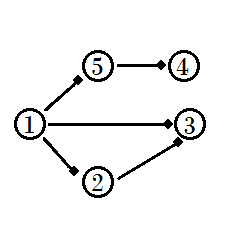
\includegraphics[scale=1]{imagenes/grafo_ejemplo_lista_ady}
			\caption{}%\label{fig:awesome_image1}
		\endminipage
		\minipage{0.55\textwidth}
			\centering
			\cppfile[6-14]{codigos/DFS.cpp}
		\endminipage
	\end{figure}	
	
	\subtitulo{DFS.}
	
	El DFS (deep first search) o Búsqueda en profundidad, es un algoritmo que permite recorrer un grafo, de manera
	general consiste en tomar un nodo, marcarlo como visitado y para cada arista hacer un llamado recursivo al nodo
	destino y repetir el proceso hasta que no queden mas nodos por visitar. Este es un algoritmo de backtraking con
	el cual se busca hacer una búsqueda completa por todos los nodos, 
	%\cppfile[26-36]{codigos/tablas_aditivas.cpp}
	
	\section{Bibliografia}
	https://es.wikipedia.org/wiki/Grafo\\
	http://trainingcamp.org.ar/anteriores/2017/clases.shtml.\\ 
	libro: competitive programming 3.\\ 



\end{document}



